% begin module arcsin-ex1
\begin{frame}
\begin{example} %[Example 1, p. 217]
\begin{columns}[t]
\column{.4\textwidth}
\[
\text{Find } \ \Arcsin \left( \frac{1}{2}\right) 
\]
\begin{itemize}
\item<2->  $\sin (\pi / 6) = 1/2$.
\item<3->  $-\pi /2 \leq \pi / 6 \leq \pi /2$.
\item<4->  Therefore $\Arcsin \left( \frac{1}{2}\right) = \frac{\pi}{6}$.
\end{itemize}
\column{.6\textwidth}
\[
\text{Find } \ \tan \left( \Arcsin \left( \frac{1}{3}\right) \right)
\]
\begin{itemize}
\item<5->  Let $\theta = \Arcsin (1/3)$, so $\sin \theta = 1/3$.
\item<6->  Draw a right triangle with opposite side $1$ and hypotenuse $3$.
\item<7->  \alert<handout:0| 7-8>{Length of adjacent side $ = \uncover<8->{\sqrt{3^2-1^2} = \sqrt{8} = 2\sqrt{2}.}$}
\item<9->  Then \alert<handout:0| 9-10>{$\tan (\Arcsin \frac13) = \uncover<10->{\frac{1}{2\sqrt{2}}.}$}
\end{itemize}
%\ \only<handout:0| -5>{%
%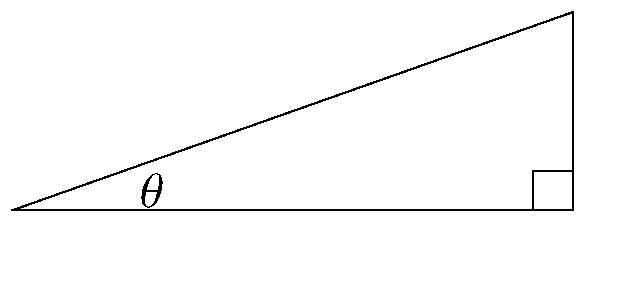
\includegraphics[width=5cm]{inverse-trig/pictures/07-06-ex1a.pdf}%
%}%
%\only<handout:0| 6-7>{%
%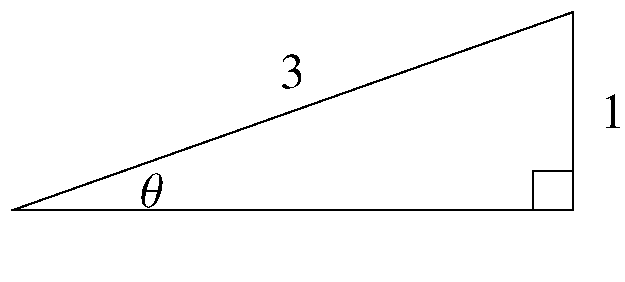
\includegraphics[width=5cm]{inverse-trig/pictures/07-06-ex1b.pdf}%
%}%
%\only<8->{%
%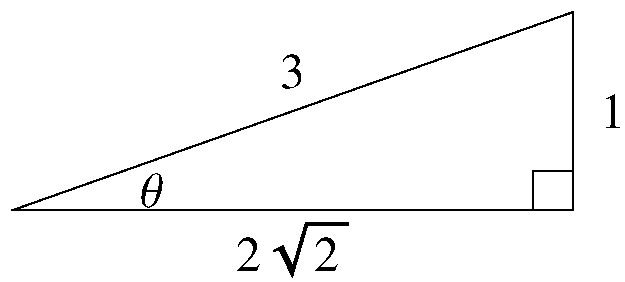
\includegraphics[width=5cm]{inverse-trig/pictures/07-06-ex1c.pdf}%
%}%
\psset{xunit=2cm, yunit=2cm}
\begin{pspicture}(-5, -5)(5,5) 
\psframe*[linecolor=white](-5,-5)(5,5) 
\uncover<5->{\psline(0,0)(2.828427125, 0)(2.828427125, 1)(0,0)
\psline(2.828427125, 0.1)(2.728427125, 0.1)(2.728427125,0)
\rput[b](1.41, 0.55){$3$}
\rput[l](2.87, 0.5){$1$}
\rput(0.55, 0.1){$\theta$}
}
\uncover<7>{\rput[t](1.41, -0.1){\alert<7>{?}} }
\uncover<8->{\rput[t](1.41, -0.1){\alert<8>{$2\sqrt{2}$}} }
\psline[linecolor=red!1](2.828427125, 1)(2.828427125, 1.1)
\psline[linecolor=red!1](0, -0.35)(0.1, -0.35)
\end{pspicture} 


\end{columns}
\end{example}
\end{frame}
% end module arcsin-ex1